% !TeX spellcheck = en_EN-English

\documentclass[12pt, twoside, openany]{book}
%\documentclass[12pt, oneside]{book}  % jednostranna tlac
\linespread{1.25} % hodnota 1.25 by mala zodpovedat 1.5 riadkovaniu
\pagestyle{plain}
% -------------------
% --- Packages
% -------------------
\usepackage[a4paper,top=2.5cm,bottom=2.5cm,left=3.5cm,right=2cm]{geometry}
\usepackage[utf8]{inputenc}
\usepackage[T1]{fontenc}
\usepackage{graphicx}
\usepackage{url}

% --- additional packages
\usepackage{epsfig}
\usepackage{epstopdf}
%\usepackage[chapter]{algorithm}
\usepackage{algorithmic}
%\usepackage{listings}
\usepackage{amsmath}
\usepackage{amssymb}
\usepackage{multirow}
\usepackage{booktabs}
\usepackage{color}
\usepackage{setspace}
\usepackage{tabularx}
\usepackage{textcomp}
\usepackage{caption}
\usepackage{natbib}
\usepackage{subcaption}
\usepackage[font=large]{subcaption}
\usepackage{emptypage}
\usepackage{float}
\usepackage[hidelinks,breaklinks]{hyperref}
%\usepackage{minted}
\usepackage[thinlines]{easytable}
\usepackage{amsmath}
\usepackage{xparse}

\NewDocumentCommand{\INTERVALINNARDS}{ m m }{
	#1 {,} #2
}
\NewDocumentCommand{\interval}{ s m >{\SplitArgument{1}{,}}m m o }{
	\IfBooleanTF{#1}{
		\left#2 \INTERVALINNARDS #3 \right#4
	}{
		\IfValueTF{#5}{
			#5{#2} \INTERVALINNARDS #3 #5{#4}
		}{
			#2 \INTERVALINNARDS #3 #4
		}
	}
}

%\captionsetup[subfigure]{font=large}

\newcommand{\mycomment}[1]{}


%aby sa nevykreslovali obrazky
%\renewcommand{\includegraphics}[2][]{
%   \fbox{#2}% print file name in a small box
%}


% -------------------
% --- Definicia zakladnych pojmov
% -------------------
\def\mfrok{2025}
\def\mftitle{Prediction of health status deterioration} % názov práce
\def\mfthesistype{Master thesis}
\def\mfauthor{Bc. Marián Kravec}
\def\mfskolitel{MSc. František Dráček}
\def\mfkonzultant{} 
\def\mfplacedate{Bratislava, 2025}
\def\mfuniversity{COMENIUS UNIVERSITY IN BRATISLAVA}
\def\mffaculty{FACULTY OF MATHEMATICS PHYSICS AND INFORMATICS}
\def\mfodbor{Applied informatics}
\def\program{Applied informatics}
\def\mfpracovisko{Department of Applied Informatics }

\begin{document}
\frontmatter


% -------------------
% --- Obalka ------
% -------------------
\thispagestyle{empty}

\noindent
\begin{minipage}{\textwidth}
    \begin{center}
        \textbf{\mfuniversity \\
        \mffaculty}
    \end{center}
\end{minipage}

\vfill
\begin{figure}[!hbt]
	\begin{center}
		
\includegraphics[width=0.4\textwidth]{images/FMFI_logo_BP.png}
		\label{img:logo}
	\end{center}
\end{figure}
\begin{center}
		\textbf{\MakeUppercase{\Large\mftitle}}\\
		\mfthesistype
\end{center}
\vfill
\mfrok \hfill
\mfauthor
%\eject 
\cleardoublepage
% --- koniec obalky ----



% -------------------
% --- Titulný list
% -------------------
\thispagestyle{empty}
\noindent
\begin{minipage}{\textwidth}
    \begin{center}
        \textbf{\mfuniversity \\
        \mffaculty}
    \end{center}
\end{minipage}

\vfill
\begin{figure}[!hbt]
    \begin{center}
        
\includegraphics[width=0.4\textwidth]{images/FMFI_logo_BP.png}
        \label{img:logo_dark}
    \end{center}
\end{figure}

\begin{center}
	\textbf{\MakeUppercase{\Large\mftitle}}\\
	\mfthesistype
\end{center}
\vfill


\begin{tabular}{l l}
Study program: & \program \\
Branch of study: & \mfodbor \\
Department: & \mfpracovisko \\
Supervisor: & \mfskolitel \\
Consultant: & \mfkonzultant \\
\end{tabular}

\vfill
\noindent
\mfplacedate \hfill
\mfauthor
%\eject 
\cleardoublepage
% --- Koniec titulnej strany



% -------------------
% --- Zadanie z AIS
% -------------------
% v tlačenej verzii s podpismi zainteresovaných osôb.
% v elektronickej verzii sa zverejňuje zadanie bez podpisov
% v pracach v naglictine anglicke aj slovenske zadanie

\newpage 
\thispagestyle{empty}
\hspace{-2cm}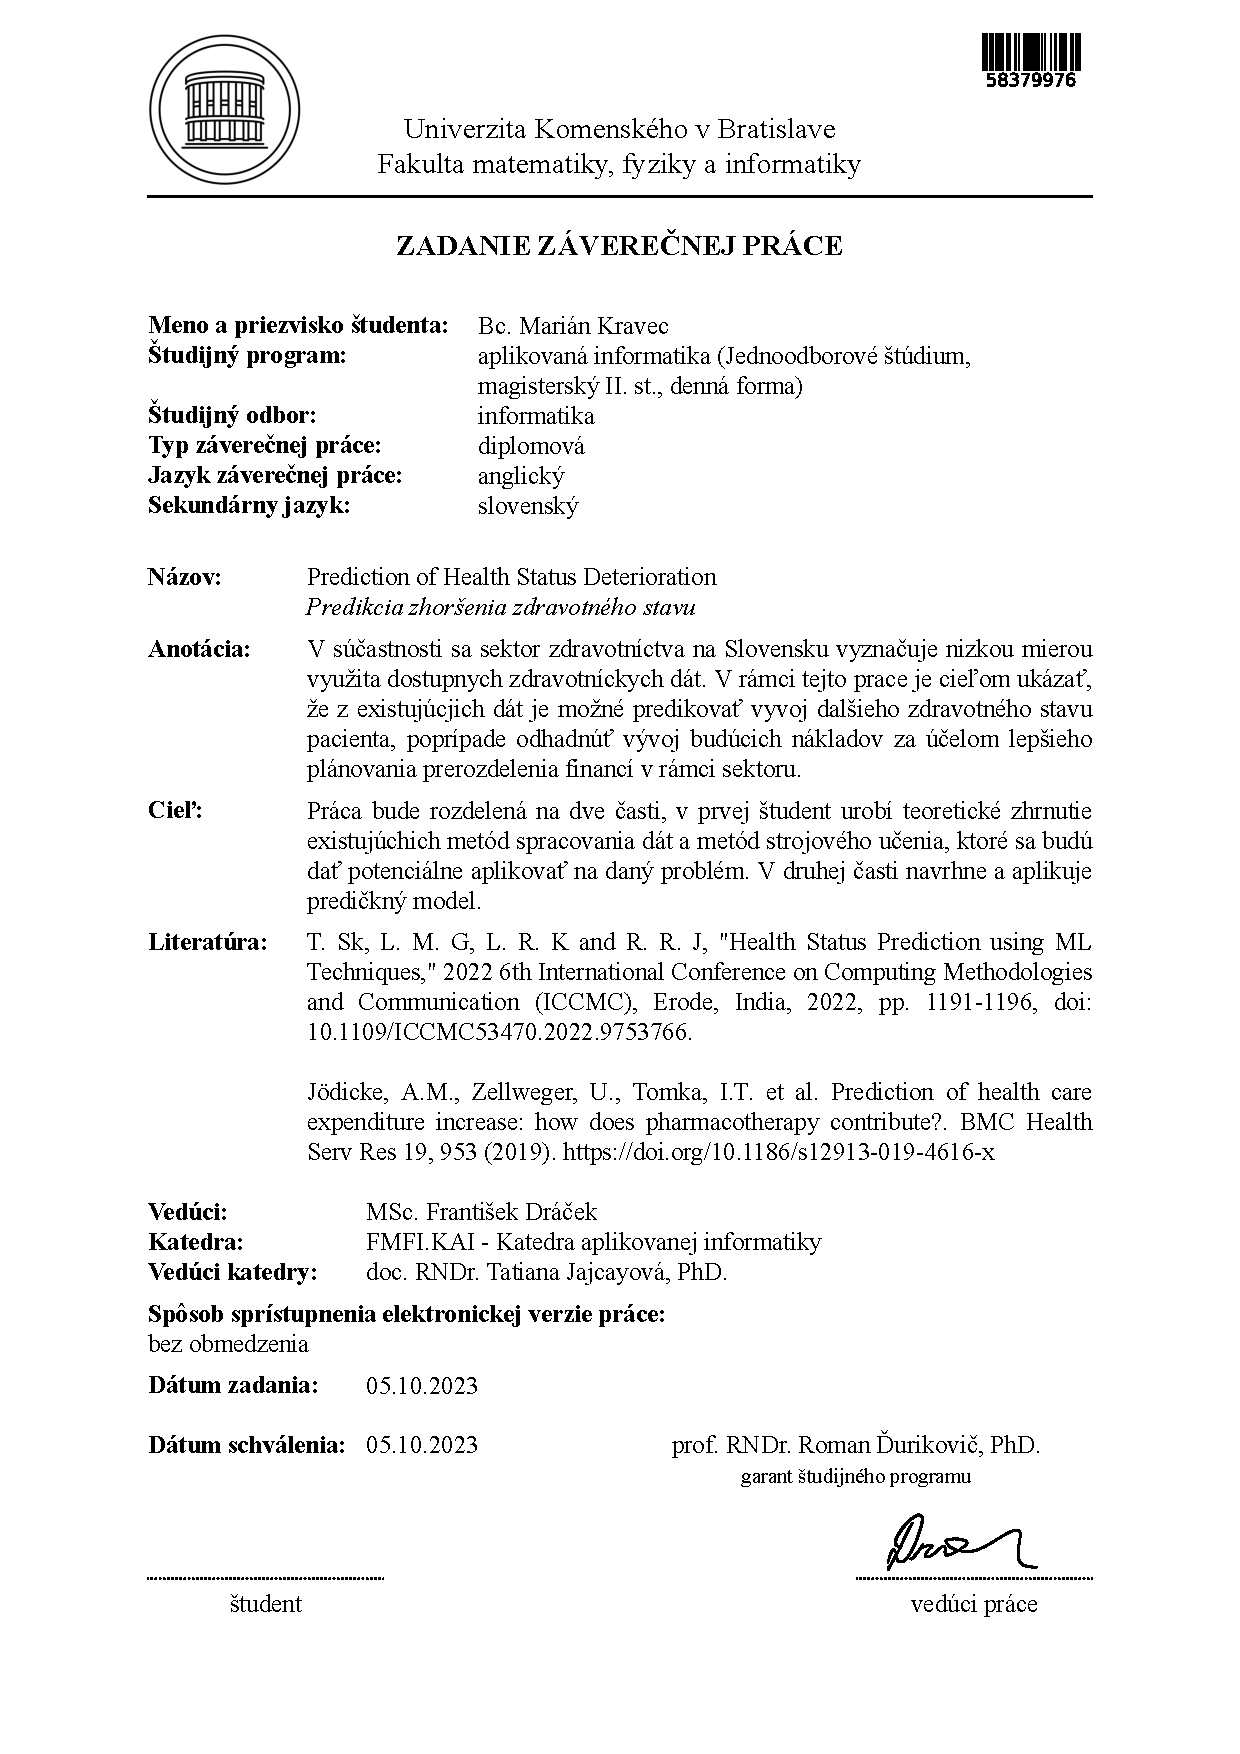
\includegraphics[page=1,width=1\textwidth]{zadaniePrace_NEW.PDF}

%\newpage 
%\thispagestyle{empty}
%\hspace{-2cm}\includegraphics[page=2,width=1\textwidth]{zadaniePrace.PDF}

% --- Koniec zadania


% -------------------
% --- Prehlásenie
% -------------------

{~}\vspace{12cm}

\noindent
\begin{minipage}{0.25\textwidth}~\end{minipage}
\thispagestyle{empty}
\begin{minipage}{0.75\textwidth}
I hereby declare that I have written this thesis by myself, only with help of referenced literature, under the careful supervision of my thesis advisor.
\newline \newline
\end{minipage}
\vfill
~ \hfill {\hbox to 6cm{\dotfill}} \\
\mfplacedate \hfill \mfauthor
\vfill\eject \cleardoublepage
% --- koniec prehlasenia




% -------------------
% --- Poďakovanie
% -------------------
\newpage
\thispagestyle{empty}
\chapter*{Acknowledgment}\label{chap:thank_you}

I would like to express my sincere gratitude to all those who supported me throughout the journey of completing this diploma thesis.
\\

First and foremost, I am deeply thankful to my supervisor, František Dráček, for his invaluable guidance, encouragement, and insightful feedback during every stage of my research. His expertise and patience have been instrumental in shaping this work.
\\

I would also like to thank the Faculty of Mathematics, Physics and Informatics at Comenius University for providing an inspiring academic environment and access to state-of-the-art research facilities. The faculty’s commitment to excellence in mathematics, physics, and informatics has greatly enriched my academic experience.
\\

Special thanks go to my colleagues and friends for their support, stimulating discussions, and for making this journey memorable.
\\

Finally, I am profoundly grateful to my family for their unwavering love, patience, and motivation. Their belief in me has been my greatest source of strength.


\vfill\eject 
% --- koniec podakovania



% -------------------
% --- Abstrakty
% -------------------
\newpage 
\thispagestyle{empty}
\chapter*{Abstract}\label{chap:abstract_en}
% !TeX spellcheck = en_EN-English

Currently, the healthcare sector in Slovakia is characterized by a low rate of utilization of available healthcare data. The aim of this work is to show that from existing data it is possible to predict the development of the patient's further health status, or to estimate the development of future costs in order to better plan the redistribution of finances within the sector.

\paragraph*{Keywords: cost prediction, patient future, transformers}  


\newpage 
\thispagestyle{empty}
\chapter*{Abstrakt}\label{chap:abstract_sk}
% !TeX spellcheck = sk_SK-Slovak

ABSTRACT SK

\paragraph*{Kľúčové slová: predikcia ceny, budúcnosť pacienta, transformery}


% --- koniec abstraktov


% -------------------
% --- Obsah
% -------------------
\newpage 
\tableofcontents

% ---  Koniec Obsahu


% -------------------
% --- Zoznamy tabuliek, obrázkov - nepovinne
% -------------------
\newpage 
\listoffigures
\listoftables
% ---  Koniec Zoznamov

% !TeX spellcheck = en_EN-English

\chapter*{Terminology}

\section*{Terms}

%\begin{itemize}
    \setlength\itemsep{1px}
    %\item \textbf{Star field tracking (sidereal)} \\
    %Ground-based tracking mode in which, telescope is moving in the same direction and speed as the apparent motion of stars.
%\end{itemize}

\section*{Abbreviations}

\begin{itemize}
    \setlength\itemsep{1px}
    \item \textbf{CPT} - Current Procedural Terminology.
    \item \textbf{EHR} - Electronic Health Records.
    \item \textbf{LLM} - Large language model. 
    \item \textbf{LaBSE} - Language-agnostic BERT sentence embedding model.
    \item \textbf{BERT} - Bidirectional encoder representations from transformers.
    \item \textbf{KNN} - K-nearest neighbors algorithm.
    \item \textbf{ICD-10-CM} - International Classification of Diseases, Tenth Revision, Clinical Modification.
    \item \textbf{MKCH-10} - International Classification of Diseases, Tenth Revision (Medzinárodná klasifikácia chorôb).
    \item \textbf{ATC} - Anatomical Therapeutic Chemical.
\end{itemize}






\mainmatter

% !TeX spellcheck = en_EN-English

%\chapter{Motivation and introduction}
\chapter*{Motivation}
% spomenut vysledky  v clanku 
% preco sme sa rozhodli spravit tuto pracu

State governments and insurance companies collect and store vast amounts of medical data, including patient histories, treatment records, prescriptions, and billing information. This data can be used for various purposes, such as detecting fraudulent activities, tracking contagious disease outbreaks, or allocating future supplies of purchased medication.
\\

Another interesting application is predicting a patient's future health, which allows for forecasts of potential diseases they may develop and the treatments they might require. Unfortunately, due to the large number of significant factors not captured in medical records, this task is almost impossible to accomplish accurately.
\\

That's why, in this study, we focus on a simpler problem: predicting the expected cost for a patient in the next year. Specifically, we aim to estimate the total anticipated costs of medications and medical procedures provided to a patient over a one-year period. In general, our approach involves two main tasks. First, we embed patient records into numerical vectors. Second, we train a model to predict each patient’s future costs based on their previous records.
\\

In the very first chapter, we briefly introduce our goal, the challenges we encountered, and the methods we used. The second chapter provides a quick overview of studies that address similar problems. The third chapter is dedicated to introducing the data we used. In the fourth chapter, we present the models and techniques employed for embedding records and for the prediction task. The fifth chapter is a brief section on the technical aspects of software design, including the programming languages and libraries we used. After that, in the sixth chapter, we describe how we implemented solutions to our two main tasks. The seventh chapter focuses on preliminary research, specifically the testing of embedding methods and various model parameters. Finally, in the eighth chapter, we discuss the results of the final model.
% !TeX spellcheck = en_EN-English

\chapter{Introduction}

In this chapter, we briefly introduce our goal, the challenges we encountered, and the methods we used.
\\

The main goal of our study is to develop software capable of analyzing patients’ historical records-specifically, the medications prescribed to them and the medical procedures they have undergone-in order to predict the cost category each patient will belong to in the following year. In other words, we aim to estimate the expected expenses for each patient over the next year based on their prior medical data. 
\\

To achieve the desired outcome, we faced three primary challenges. First, we needed to transform patients' historical records into numerical vectors suitable as input for machine learning models. Second, we had to simulate patients' potential futures by predicting both likely medication prescriptions and medical procedures they might undergo in the subsequent year. Finally, we required a method to calculate the expected costs of these projected treatments and aggregate them into an annual cost estimate for each patient.
\\

For record transformation (referred to as embedding later in the study), we focused on embedding medications, diagnoses, and medical procedures. We employed one of two methods depending on whether the data contained structured codes. When structured codes were available, we split the code into its hierarchical components, embedded each part individually, and then combined the results to create a comprehensive representation. For data without structured codes or meaningful organization, we utilized a machine learning-based language model to generate embeddings directly from textual descriptions.
\newpage

To generate future medical records, we evaluated several sequential data models, including LSTM (Long Short-Term Memory) networks and decoder-only Transformer architectures, as patients' future medications and procedures exhibit strong temporal dependencies on their historical records, with recent events carrying greater predictive weight.
\\

To estimate the cost category of each medical record, we primarily utilized a Multi-layer Perceptron (MLP) model. This neural network takes the numerical representation of a record (generated through our embedding process) as input and predicts its likely cost category. While the MLP served as our core approach, we also explored alternative models such as Gradient Boosting and Ridge Regression for comparative analysis.
\\

After resolving the three key challenges we integrated these components into a unified software solution. This final system sequentially processes patient histories through each stage to generate annual expense forecasts.

% !TeX spellcheck = en_EN-English

\chapter{Similar studies}

% !TeX spellcheck = en_EN-English

One of sub-task for prediction of patient future is to group medical procedures into clusters because there are many procedures that even thought have different codes they are essentially same or similar enough that leaving them separate would only cause issue for predicting model.

For this task Lorenzi et al. from Duke University in Durham developed novel algorithm called Predictive Hierarchical Clustering \cite{lorenzi2017predictive}. This algorithm was developed for agglomerative clustering of surgical CPT codes. This algorithm uses one-pass bottom-up approach where they utilize EHR, more precisely using 317 predictors like lab values and patients history, excluding CPT information for 3,723,252 patients and 3,132 CPT codes where each patient have one main surgical CPT code. For each CPT code then they create tree containing patients with that code. Then at each iteration, the algorithm considers merging all pairs of existing trees. To compare two trees they utilize two hypothesis, first hypothesis say that data in both trees are generated from same model, while second say data in each tree is generated from models with different parameters. Final value is weighted average of probabilities of these two hypothesis considering data in trees, where weigth is probability of first hypothesis \ref{hierClust}.

\begin{equation}
	\label{hierClust}
	p(D_k \vert T_k) = p(H_1^k)p(D_k \vert H_1^k) + (1 - p(H_1^k))p(D_i \vert T_i)p(D_j \vert T_j)
\end{equation} 

Where $D_k$ is set of data in merged tree (merged $T_i$ and $T_j$), $T_k$ is merged tree, $H_1^k$ is first hypothesis, $D_i$ and $D_j$ are data in trees $T_i$ and $T_j$. %pridavanie pod casti
% !TeX spellcheck = en_EN-English

From perspective of prediction of patient future one of similar studies is study called Deep Patient by Riccardo Miotto et al. \cite{miotto2016deep} where they were predicting which disease would patient have in the future based on his current state. Their input data were contained general demographic details such as age, gender and race, and common clinical descriptors such as diagnoses, medications, procedures, and lab tests. To predict future diseases they use random forest model with one-vs.-all learning. Study focus primarily on improving results of model by reducing noise in data by reducing their dimensionality. They compared standard approaches like principle component analysis, Gaussian mixture model or K-means, but main focus was approach using stack of denoising autoencoders. Model using stack of denoising autoencoders to reduce dimension showed significantly better results compared to both model using original dataset and models using other dimensionality reduction techniques.
\\

Another similar study, is study by Caballer-Tarazona er al. \cite{caballer2019predicting} in which they tried to predict future cost of the patient primarily using what they called "Aggregated Clinical Risk Group 3" computed from standardized Clinical Risk Group (CRG). This variable consist of the parts, first in one of nine grouped CRGs and second part is one of six levels of severity.



% !TeX spellcheck = en_EN-English

\chapter{Medical data} \label{chap:data}

To train and verify model we used anonymized data obtained from Slovak National health information center also known under abbreviation NCZI. Our data consisted of two dataset:
\begin{itemize}
	\item Records of medical procedures from ambulatory health care
	\item Records of prescribed medicines
\end{itemize}

\section{Records of medical procedures from ambulatory health care}

Each row in this dataset contains information about single medical procedure done to patient. Each record consist of these variable:
\begin{itemize}
	\item date of the procedure - date when procedure was performed
	\item code of the patient - identification code unique for the patient
	\item age of the patient - age of the patient at the time of procedure
	\item gender of the patient
	\item code of the diagnosis - identification code unique for the diagnosis for which procedure was prescribed
	\item code of the procedure - identification code unique for the medical procedure 
	\item cost of the procedure - cost associated with performing of the procedure
\end{itemize}

For our prediction we use most of these information, date of the procedure combined with patient age is used to create timestamp information used to order all records for patient as well as one of the dimension of record embedding. Identification code of patient is used to be able to gather all records for single patient. Identification codes for diagnosis and procedure are matched with their corresponding numerical vector and embedded into vector corresponding to record (see \ref{embedding}). Cost is encoded into cost category and used as information of cost associated with embedding of record.

\section{Records of prescribed medicines}

Similarly to dataset containing procedures, each row of this dataset contains informations about single prescription of drug to specific patient.  Each record consist of these variable:
\begin{itemize}
	\item date of the prescription - date when drug was prescribed
	\item code of the patient - identification code unique for the patient
	\item age of the patient - age of the patient at the time of procedure
	\item gender of the patient
	\item code of the diagnosis - identification code unique for the diagnosis for which drug was prescribed
	\item code of the drug - identification code unique for the medical procedure 
	\item cost of the drug - cost associated with performing of the procedure
\end{itemize}

Use of these variable is also similar to procedures, with only difference that instead of using encoding procedure into record embedding we encode drug.

\mycomment{
EQUATION SHOWCASE:
\begin{equation}
	\label{eqn:starskynoise}
	\sigma_{star} = \sqrt{S_{star}} \quad \sigma_{sky} = \sqrt{S_{sky}}
\end{equation} 

FIGURE SHOWCASE:
\begin{figure}[!h]
	\centering
	\begin{subfigure}{.3\textwidth}
		\centering
		
\includegraphics[width=\textwidth]{images/FMFI_logo_BP.png}
		\caption{Hot pixels.}
		\label{fig:hotpixels}
	\end{subfigure}
	\begin{subfigure}{.3\textwidth}
		\centering
		
\includegraphics[width=\textwidth]{images/FMFI_logo_BP.png}
		\caption{Dead columns.}
		\label{fig:deadcolumns}
	\end{subfigure}
	
	\vspace*{4mm}
	
	\begin{subfigure}{.3\textwidth}
		\centering
		
\includegraphics[width=\textwidth]{images/FMFI_logo_BP.png}
		\caption{Traps.}
		\label{fig:trap}
	\end{subfigure}
	\begin{subfigure}{.3\textwidth}
		\centering
		
\includegraphics[width=\textwidth]{images/FMFI_logo_BP.png}
		\caption{Saturation trail.}
		\label{fig:saturationtrail}
	\end{subfigure}
	\caption{Examples of some internal defects present on FITS images acquired by AGO70.}
	\label{fig:internaldefects}
\end{figure}
}
% !TeX spellcheck = en_EN-English

\chapter{Theory - models}
\label{chap:thoery}

During our research, we utilized several different machine learning models. In this chapter, we introduce these models from a more theoretical point of view.

\section{Multilayer perceptron}
\label{MLP}

A multilayer perceptron is a feed-forward neural network, meaning that data flows in a single direction and neurons do not form cycles. This network consists of fully connected, sometimes called dense, layers with non-linear activation functions, as shown in Fig. \ref{fig:mlp}. We can see that this model can be split into three parts: the input layer, which loads the data; the hidden layers, which extract the desired information using linear transformations and activation functions; and finally, the output layer, which applies a final linear transformation followed by an activation function to produce the output. Each layer can be described using the formula shown in Eq. \ref{eqn:mlp}, where $h_i$ is the resulting vector of the $i$-th layer, $act()$ is a non-linear activation function, $W_i$ is the weight matrix of the $i$-th layer, $h_{i-1}$ is the resulting vector from the previous layer, and $b_i$ is the bias vector.

\begin{equation}
	\label{eqn:mlp}
	h_i = act(W_i h_{i-1} + b_i),
\end{equation}

\begin{figure}[!h]
	\centering
	
	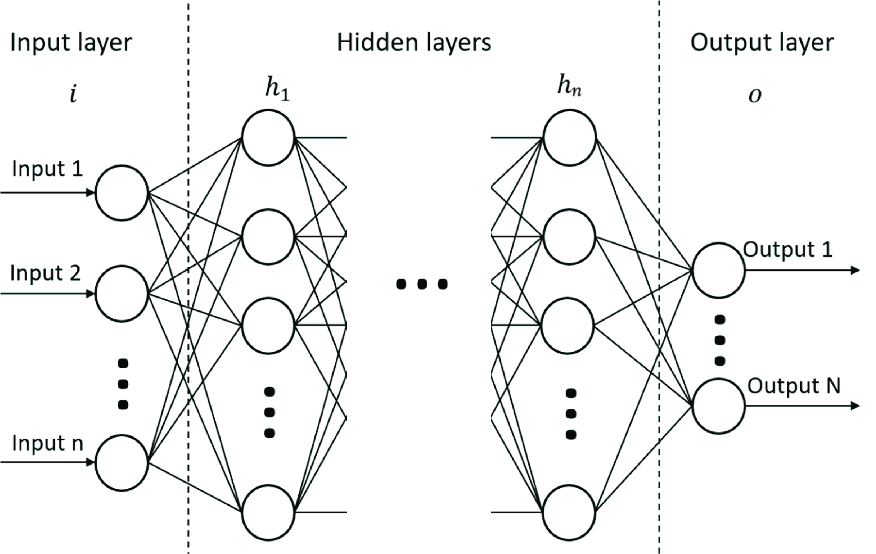
\includegraphics[width=0.8\textwidth]{images/MLP_arch.png}
	
	\caption{Architecture of multilayer perceptron \cite{MLParch}.}
	\label{fig:mlp}
\end{figure} 

\section{Recurrent neural network}
\label{theoryRNN}

In general, a recurrent neural network is a type of neural network that, in some way, uses results from previous steps to improve its predictions. These models are used for ordered data, where each subsequent step depends on more than just the immediately preceding one.

\subsection{Elman RNN}

The Elman RNN, also known as a simple recurrent network (SRN), is a type of recurrent neural network that utilizes the results of the hidden layer before activation in the previous step as an additional input in the next one. We can see this architecture in Fig. \ref{fig:elman_arch}, where on the left we observe how forward propagation occurs and on the right how it is unrolled over time. Here, the middle layer, which is the hidden layer of the model, receives two inputs: the input vector $x_t$, where $t$ denotes the step (usually a time step), which is multiplied by a matrix of weights $W_i$, and the vector $h_{t-1}$, which is the result of this layer (also called the context vector) from the previous step, multiplied by a different matrix of weights denoted as $W$. These two results are summed together, and the result is passed to the activation layer, which generates the new vector $h_t$ \cite{elman}. This entire process is summarized in Eq. \ref{eqn:elman}, where $b_i$ and $b$ are bias vectors.

\begin{equation}
	\label{eqn:elman}
	h_t = act(x_t W^T_i + b_i + h_{t-1} W^T + b).
\end{equation} 

Usually, this result is directly used as the output or passed through a single fully-connected feed-forward layer. In a multi-layered version of this network, the output of the first hidden layer is fed into the next hidden layer, along with the output of that specific layer from the previous step. Both inputs are multiplied by weight matrices specific to that layer, summed together, and then passed through an activation function.

\begin{figure}[!h]
	\centering
	
	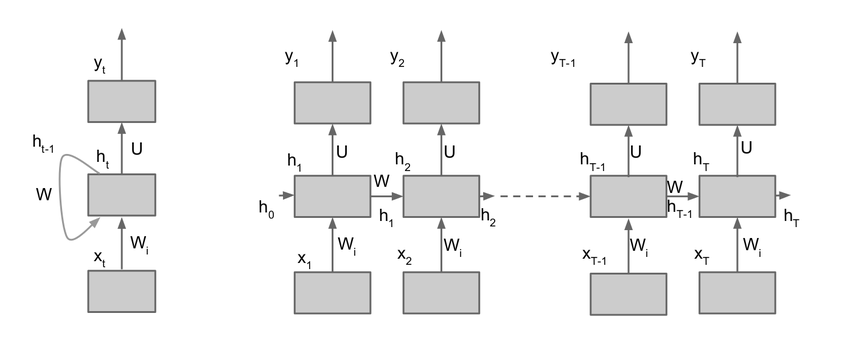
\includegraphics[width=0.85\textwidth]{images/Elman_RNN_architecture.png}
	
	\caption{Architecture of Elman RNN \cite{elman_img}.}
	\label{fig:elman_arch}
\end{figure}

\subsection{Gated Recurrent Unit}

A Gated Recurrent Unit (GRU) is a more complex RNN variant compared to the Elman RNN. Developed as a simplification of the even more intricate LSTM model, the GRU primarily consists of three interacting components: the reset gate, update gate, and candidate hidden state computation. These components collaboratively regulate information flow to produce the final prediction.
\\

The structure of a GRU’s hidden layer is illustrated in Fig. \ref{fig:gru_arch}. In this diagram:

\begin{itemize}
	\item Sigmoid: Represents a fully connected feed-forward layer with a sigmoid activation function.
	\item Tanh: Represents a fully connected feed-forward layer with a hyperbolic tangent activation function.
\end{itemize}

The reset gate, located on the left side of the diagram, uses the input and previous hidden state vectors to modify the previous hidden state vector, which is then fed into the candidate hidden state computation. This process helps capture short-term dependencies in time series by selectively removing information from the previous hidden state vector.
\\

The candidate hidden state computation is similar to the Elman RNN but with two key differences: first, the inputted hidden layer is modified by the reset gate's result; second, the resulting vector from this part serves only as a candidate that undergoes further calculation. This candidate vector primarily contains current and short-term past information due to the specific vectors that form its input.
\\

The update gate, similar to the reset gate, uses the concatenation of the input and previous hidden state vector as its input. However, its results are used to modify both the previous hidden state and the candidate hidden state, creating a final hidden state that is a weighted average of these two vectors, with weights derived from this gate. This architecture helps capture long-term dependencies in time series by reintroducing relevant information from the previous hidden state vector into the final hidden state, combining it with the candidate hidden state vector that contains mostly current and short-term information. The entire architecture is depicted in Fig. \ref{fig:gru_arch}.
\\

\begin{figure}[!h]
	\centering
	
	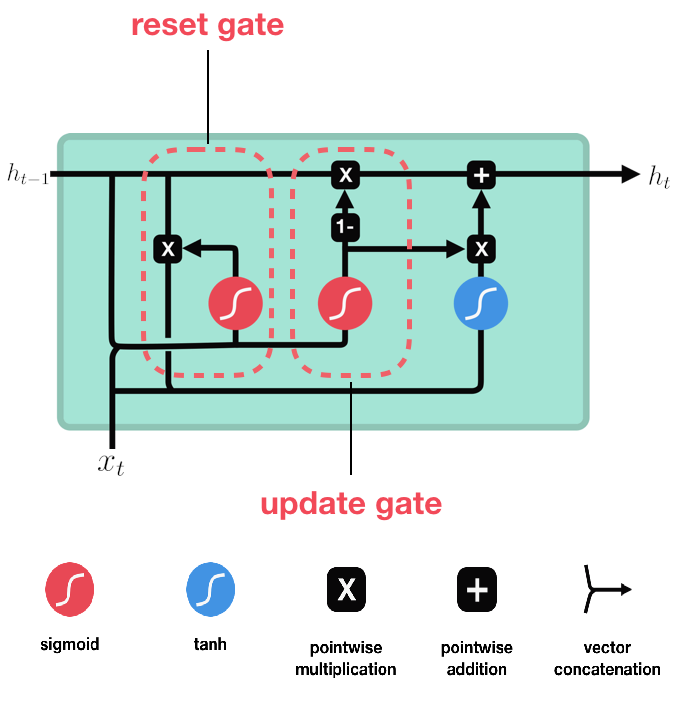
\includegraphics[width=0.6\textwidth]{images/GRU_arch.png}
	
	\caption{Architecture of GRU hidden layer.}
	\label{fig:gru_arch}
\end{figure}

The multi-layered version of this architecture is achieved by stacking hidden layers, where the hidden state vector of one layer becomes the input vector for the next.

\subsection{Long Short-Term Memory}

As mentioned earlier, the LSTM is a more complex predecessor of the GRU. Developed to address the vanishing gradient problem that limits long-term memory in models like the Elman RNN, the LSTM introduces a memory vector, often called a memory cell, designed to maintain information over longer periods. As shown in Fig. \ref{fig:lstm_arch}, this model consists of three gates and a candidate memory computation. The legend in this diagram has the same meaning as in the GRU architecture diagram.
\\

All three gates and the candidate memory computation share the same input, which consists of the input vector and the previous hidden state vector. In each case, this input passes through a fully connected feed-forward layer and then into an activation function. For the gates, this activation function is the sigmoid function, which bounds all values within the range (0,1), while the candidate memory calculation uses the hyperbolic tangent as its activation function.
\\

The forget gate is responsible for removing unnecessary information from the memory vector by performing an element-wise multiplication of its result with the previous memory vector.
\\

The input gate, together with the candidate memory vector computation, is designed to introduce new information into the memory cell after adjustments made by the forget gate. First, the model computes the candidate memory vector; this vector is then adjusted by the input gate's result and added to the modified previous memory vector, resulting in a new memory vector.
\\

Finally, the output gate determines how much each part of the memory should contribute to the new hidden state vector. This process is illustrated in Fig. \ref{fig:lstm_arch}.

\begin{figure}[!h]
	\centering
	
	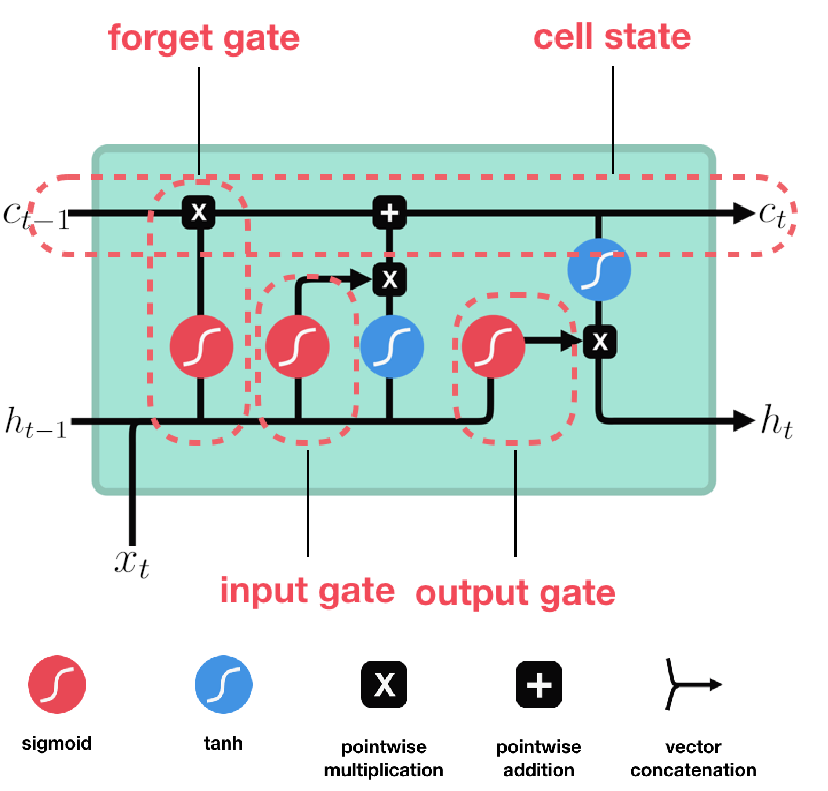
\includegraphics[width=0.6\textwidth]{images/LSTM_arch.png}
	
	\caption{Architecture of LSTM hidden layer.}
	\label{fig:lstm_arch}
\end{figure}
\newpage

\section{Transformer}
\label{theoryTrans}

The Transformer is a deep learning model architecture introduced in 2017 by Vaswani et al. \cite{attentionAllYouNeed} that is especially good at handling sequences, such as text. This architecture consists of an encoder and a decoder, as shown in Fig. \ref{fig:trans}. The encoder in this model is meant to create a contextualized representation of the input, while the decoder takes this contextualized representation and combines it with previous outputs to predict the next output. In addition to these two main blocks, this model usually also contains a tokenizer, an embedding layer, and positional encoding to prepare the input data, as well as a fully connected feed-forward layer with a softmax activation function to turn the result of the decoder into a probability distribution over possible tokens.

\begin{figure}[!h]
	\centering
	
	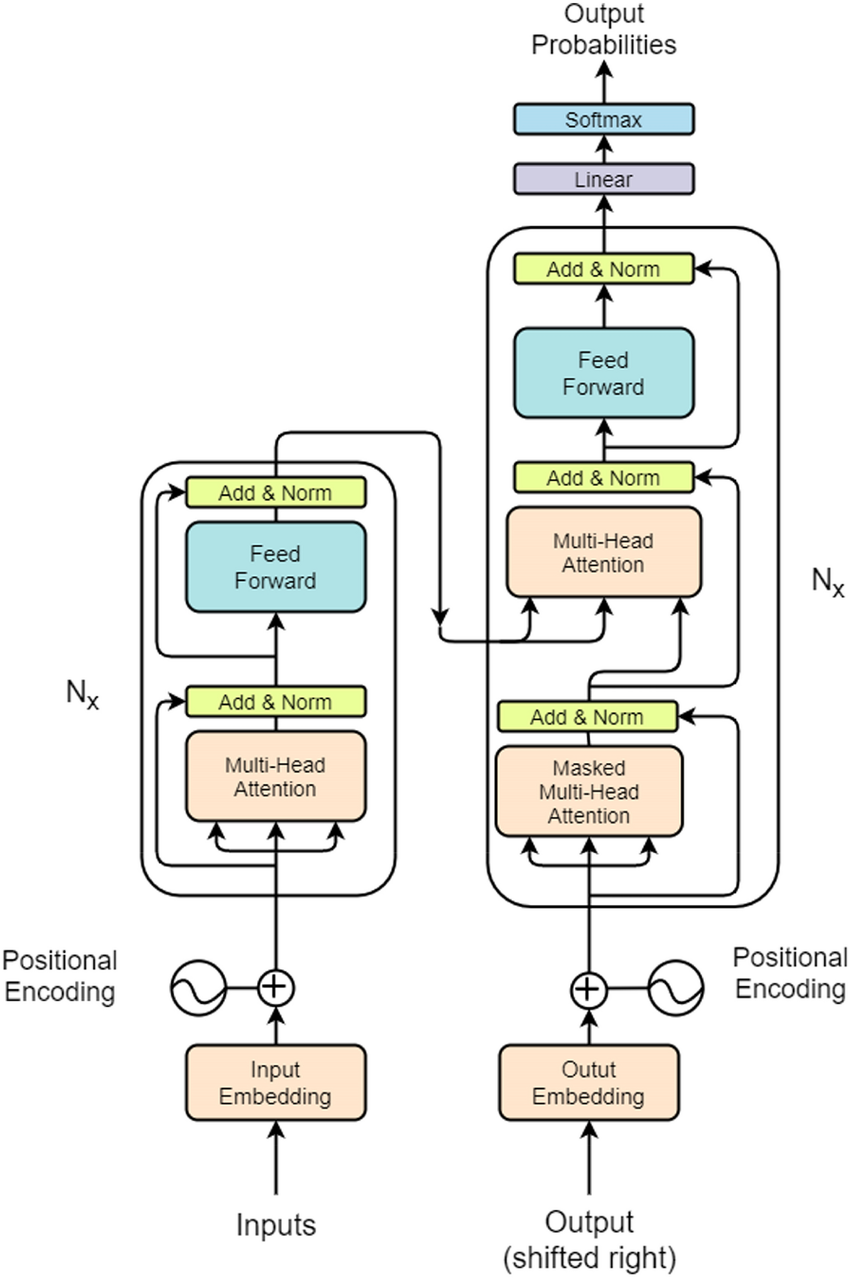
\includegraphics[width=0.6\textwidth]{images/trans_arch.png}
	
	\caption{Architecture of one encoder-decoder block in transformer model from original "Attention is all you need" paper \cite{attentionAllYouNeed}.}
	\label{fig:trans}
\end{figure}

\subsection{Tokenizer, Embedding layer and Positional encoding}

The first part of the Transformer model is usually input preparation, which may vary depending on the type of data used. This part consists of three components:

\begin{itemize}
	\item Tokenizer: This layer splits the input into tokens. For example, if the input is textual, tokens might be words or syllables.
	\item Embedding layer: The task of this layer is to transform each input token into a numerical vector of the same length.
	\item Positional encoding: The final preparation layer adds a vector to each token’s embedding, encoding its position relative to other tokens.
\end{itemize}

In most cases, the Tokenizer and Embedding layer are trained separately and do not change during training of the Transformer, while the Positional Encoding is trained alongside the rest of the Transformer.

\subsection{Encoder}
\label{theoryEncoder}

Encoder architecture consists of multiple attention blocks, where each block consists of multi-headed self-attention and a multi-layered feed-forward neural network. After each of these steps, the embeddings from the step input are added to the output, and the result is layer-normalized. Adding the step input embedding creates residual paths that help mainly with the vanishing gradient problem, while layer normalization ensures that the results neither explode nor vanish, and also brings a bit of additional non-linearity to the model. First, input embeddings are split into parts, each of which goes into a separate self-attention head.
\\

The architecture of self-attention is shown in Fig.~\ref{fig:self_att}, where we can see that each input token is multiplied by key, query, and value matrices to obtain their key, query, and value vectors. After that, each query is multiplied with each key to create the attention matrix, which encodes how much each token influences the others. This matrix then goes into a column-wise softmax function to normalize it, and finally, it is multiplied by the matrix of value vectors to create new embeddings of the tokens that should contain not only the original information but also the influence information.
\\

\begin{figure}[!h]
	\centering
	
	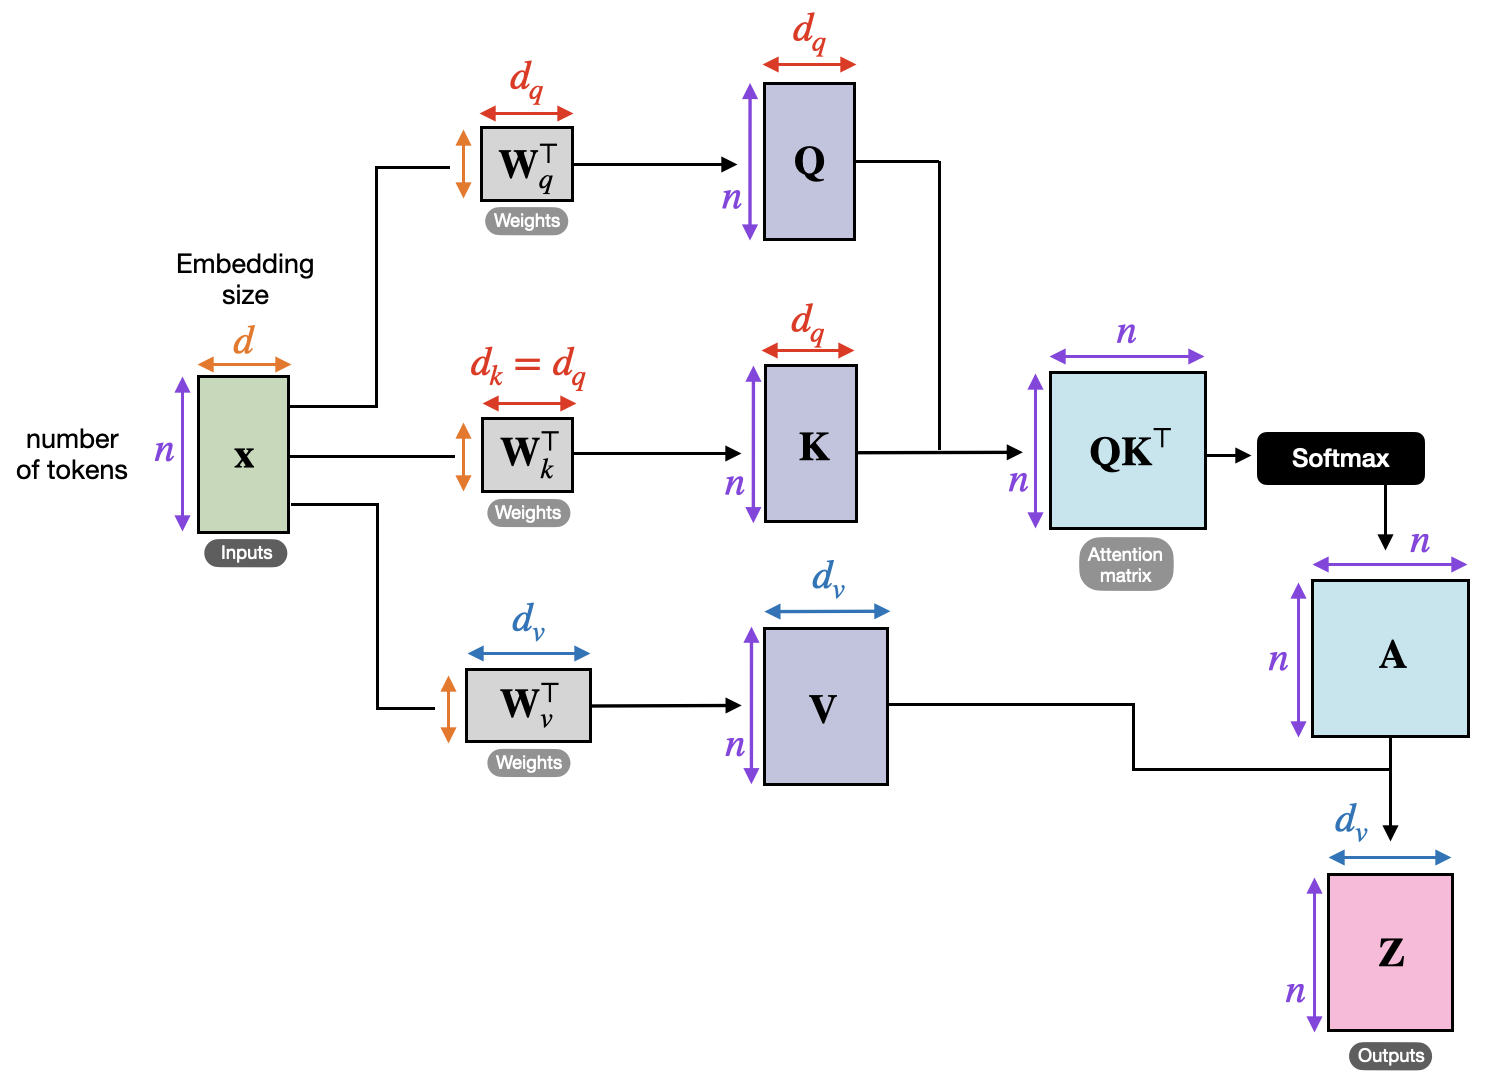
\includegraphics[width=1\textwidth]{images/self_attention.png}
	
	\caption{Architecture of Self-attention mechanism.}
	\label{fig:self_att}
\end{figure}

The results of each self-attention head are then concatenated back into new embeddings that have the same dimensions as the original ones. After adding the residual connection and normalization, the results go into a multi-layered feed-forward neural network to further extract information from the embeddings.

\subsection{Decoder}

The architecture of the decoder, similarly to the encoder, consists of multiple attention blocks; however, in this case, each attention block consists of three parts instead of two.
\\

The first part is masked multi-headed self-attention, which is similar to unmasked self-attention, with the only difference being the application of masking to the attention matrix before the softmax function. This ensures that words at certain positions do not affect words at other specific positions. The decoder uses what is called causal or look-ahead masking, which prevents future tokens from affecting past ones. In our case, this guarantees that a record cannot be influenced by records that occur later, that is, in the future from its perspective.
\\

The second part is multi-headed cross-attention, which takes two lists of token embeddings and computes the effect of tokens in the first list on tokens in the second list. In this case, the key and value vectors are computed from the contextualized representation produced by the encoder, while the query vectors are computed from the results of self-attention in the decoder. Other than this, the remaining architecture is the same as unmasked self-attention.
\\

The final part of the decoder attention block is a multi-layered feed-forward neural network that further extracts information from the embeddings.

\subsection{Fully-connected Feed-forward layer}

After that, the results of the decoder pass into the final fully-connected feed-forward layer, which changes the dimensionality of the decoder output from the embedding size to the vocabulary size and applies a softmax activation to the result. This setup is designed to produce a probability distribution over all possible tokens for the last token.
\\

In our case, we modified this final step. We encountered a problem where most records (our tokens) were unique, creating an extremely large vocabulary. This issue arose partially due to the many possible combinations of diseases, drugs, and medical procedures encoded in each record, and partially due to timestamps adding uniqueness, as it is unlikely for two patients to receive the same drug for the same disease at the same age.
\\

To address this, we removed the softmax activation and altered the fully-connected feed-forward layer so that the result maintains the embedding dimension. We then added a function that splits the result, finds the closest embedding for each part, and concatenates these embeddings together, yielding a specific new embedding prediction instead of a probability distribution.

\subsection{Decoder-only Transformer}

The Decoder-only version of the Transformer model is a simplified variant that entirely excludes the Encoder part and removes the Cross-Attention mechanism from the Decoder. This model is typically used when generating subsequent tokens without relying on a stable contextual input that would normally be processed by the Encoder.
\\

This simplification makes the architecture more akin to a standard RNN in terms of input-output behavior, where the model generates sequences step-by-step without explicit cross-contextual dependencies.

\section{Language-agnostic BERT Sentence Embedding}
\label{theoryLaBSE}

The Language-agnostic BERT Sentence Embedding model, also known as LaBSE, is a model trained with the main goal of generating similar representations for pairs of sentences that have the same meaning and are only translations of each other in two different languages \cite{labse_kaggle}.
\\

The architecture of the LaBSE model consists of four parts \cite{labse_hug}:

\begin{enumerate}
	\item Encoder-only transformer (BERT model)
	\item Pooling layer
	\item Dense layer
	\item Normalization layer
\end{enumerate}

\subsection{Encoder-only Transformer (BERT model)}
\label{emb:trans}

The first and most important part of the LaBSE model is the transformer, a deep learning architecture. More specifically, LaBSE uses BERT (Bidirectional Encoder Representations from Transformers), an encoder-only transformer architecture. This means the model lacks the decoder found in the standard Transformer (typically used for prediction tasks), allowing BERT to focus solely on extracting contextual information from input text.
\\

The architecture of the standard BERT model includes:

\begin{enumerate}
	\item Tokenizer layer
	\item Embedding layer
	\item Encoder
	\item Task layer
\end{enumerate}

\subsubsection{Tokenizer layer}

The first layer is the tokenizer, which takes the input text and splits it into tokens. In the case of the BERT model, this is called the PieceWise tokenizer, which splits text into subwords, something similar to syllables. The PieceWise tokenizer has advantages compared to other tokenizers that use either words or characters. Compared to character-wise tokenization, subwords contain more information than individual characters. Compared to word tokenization, there are far fewer subwords than words, and subwords are more similar across multiple languages, resulting in a much smaller vocabulary. This is especially important for multilingual models. After splitting, this layer assigns an integer number to each unique token. The LaBSE model’s vocabulary distinguishes around 500,000 different tokens.

\subsubsection{Embedding layer}

After that comes the embedding layer, which assigns a real-number vector to each token. Specifically, the BERT model computes three distinct embeddings, sums them, and normalizes the result to produce the final embedding:

\begin{itemize}
	\item Token type embedding: The base embedding where each token in the vocabulary is assigned a unique vector.
	\item Positional embedding: Encodes the token’s position within the sequence, providing contextual information about its location.
	\item Segment type embedding: Indicates which segment (typically a sentence) the token belongs to, crucial for processing multi-sentence input.
\end{itemize}

\subsubsection{Encoder}

The third and most important layer is the encoder. This is the layer in which contextual information is mined from the text. The architecture of this layer is the same as the encoder described in Sec. \ref{theoryEncoder}. In the BERT variant used by LaBSE, the encoder contains 12 attention blocks.

\subsubsection{Task layer}

The training process of the BERT model usually consists of two tasks on which the model is trained at the same time. The first is Masked Language Modeling (MLM), where 15\% of input tokens are masked, meaning they are either replaced by a mask placeholder or by a random different token. The masked input then goes into the model, and the resulting tokens at the positions of the masked tokens in the input are compared to the correct tokens before masking. This creates an error that is back-propagated through the model, updating its parameters \cite{bert_pretr_1}. The other task usually used is called Next Sentence Prediction (NSP). In this task, the model receives input that starts with a special classification token and then two spans of text separated by a special separator token. The task of the model is to determine whether these two spans of text can appear one after another, or more precisely, whether they appeared consecutively in the training corpus. This information is encoded in the first token of the result using two special tokens, either "is next" or "not next." Similarly, the difference between the expected and resulting first token creates an error that is back-propagated through the model \cite{bert_pretr_2}.
\\

However, in some BERT-based models like LaBSE, the second task is replaced with Translation Language Modeling (TLM). This task is an extension of MLM, in which the model receives two concatenated sentences instead of one, where the second sentence is a translation of the first in another language. The rest of the task is the same as in MLM: the whole input is masked, and the model is tasked with predicting the masked tokens \cite{bert_pretr_3}. 
\\

The task layer is used primarily only during pre-training and is omitted when the model is used for a different task, as many use cases do not need tokens in the results but instead use embeddings from the encoding layer as a form of text encoding, which is then used in task-specific layers for fine-tuning.


\subsection{Pooling layer}

After the BERT model returns embeddings for all input tokens, these embeddings need to be aggregated into a single vector that represents the embedding of the entire input. This aggregation is typically performed using a pooling layer. In the case of LaBSE, this pooling is done simply by taking the embedding of the first token, which is the embedding of the special classification token added to the beginning of the BERT input.

\subsection{Dense layer}

The next layer is a standard feed-forward dense layer using a hyperbolic tangent activation function. The number of input and output neurons is the same, and the layer includes an additional bias neuron.

\subsection{Normalization layer}

The final layer is normalization, whose task is to normalize the resulting vector by dividing it by its $L_2$ norm, ensuring the final vector has an $L_2$ norm equal to one.

\section{Word2vec model}
\label{theoryW2v}

Word2vec is a neural network-based method for generating word embeddings, which are dense vector representations of words that capture their semantic meaning and relationships. In other words, properties like the distance between two embeddings contain underlying information about those words, such as their similarity. There are two main approaches to implementing Word2vec:

\begin{itemize}
	\item Continuous bag-of-words (CBOW) 
	\item Skip-gram
\end{itemize}

\subsection{CBOW approach}

A model using the CBOW approach receives a sequence of words called the context, with one word missing, and tries to predict the missing target word as output. The model initially assigns one-hot encoding to each word in its dictionary. During training, each word from the context is first converted into its one-hot encoded embedding, which is then multiplied by a weight matrix to obtain its lower-dimensional dense embedding. The dense embeddings of all words in the context are then averaged, and the resulting embedding goes into a hidden layer, which transforms the vector back into the dimension of the vocabulary. Finally, a softmax function is applied to get the probability of each word in the vocabulary being predicted as the missing word. We can see this architecture in Fig. \ref{fig:cbow_arch}. Training is usually done using a fixed context window moving along the training text.

\begin{figure}[!h]
	\centering
	
	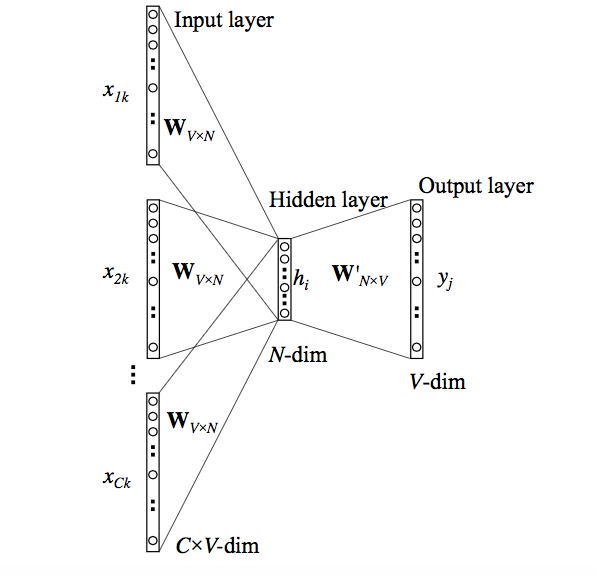
\includegraphics[width=0.9\textwidth]{images/CBOW_arch.png}
	
	\caption{Architecture of NN to train CBOW implementation of Word2vec model \cite{cbow}.}
	\label{fig:cbow_arch}
\end{figure}

\subsection{Skip-gram approach}

The Skip-gram approach works in the opposite way, the model receives a target word and tries to predict the surrounding context words. Similar to CBOW, the input word is first one-hot encoded and then multiplied by a weight matrix to transform it into a dense embedding. This embedding is passed to the next layer, which transforms it back into the vocabulary dimension. A softmax function is then applied to generate a probability distribution over potential context words.
\\

The Skip-gram’s loss function is the sum of the negative log-likelihoods of all context words. This architecture is illustrated in Fig. \ref{fig:skip_arch}.
\begin{figure}[!h]
	\centering
	
	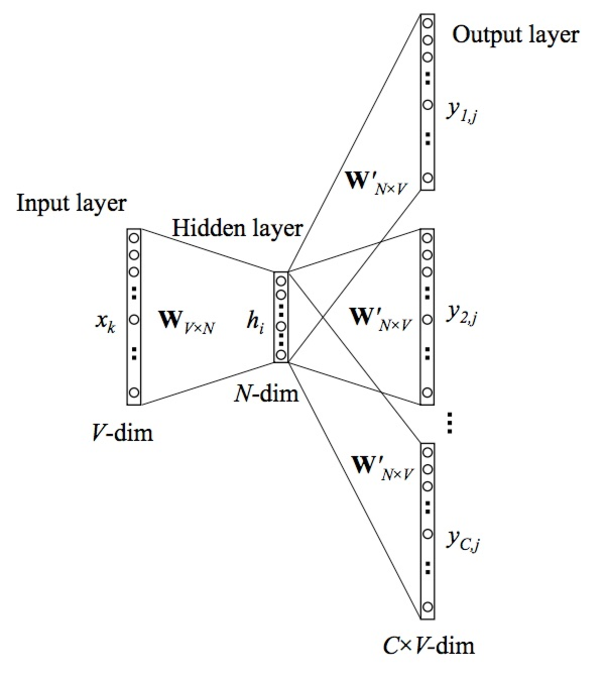
\includegraphics[width=0.9\textwidth]{images/Skip_arch.png}
	
	\caption{Architecture of NN to train Skip-gram implementation of Word2vec model \cite{skipgram}}
	\label{fig:skip_arch}
\end{figure}
% !TeX spellcheck = en_EN-English

\chapter{Proposed Methods}

Task of predicting future cost of a patient can be split input multiple sub-tasks which follow each other. The sub-tasks are these:

\begin{enumerate}
	\item Embed patient history into numerical vectors
	\item Compute expected number of records patient would have in next year
	\item Predict future records for patient
	\item Predict cost of each future record
	\item Complete total cost of patient for next year
\end{enumerate}


% !TeX spellcheck = en_EN-English

\section{Embedding of Patient}
\label{embedding}

The first sub-task in predicting a patient’s future costs is to embed each patient record into a numerical vector that can be interpreted by a neural network. Our main goal was to create embeddings that retain similarity information-meaning that records with similar diagnoses, drugs, and medical procedures receive similar embeddings. We define similarity using the Euclidean distance between embedding vectors. Preserving similarity is important because it simplifies the prediction task: the model only needs to predict a closely related record, rather than the exact one.
\\

For each patient record, we embed four distinct attributes. The first, and simplest to implement, is the timestamp, which is calculated using numerical and date values. The remaining three attributes, which are diagnosis, medical procedure, and prescribed drug, are more complex to embed.

\subsection{Timestamp}

The attribute we refer to as the timestamp of a patient’s record can be more precisely described as an approximation of the patient’s age at the time of either a medical procedure or drug prescription. This timestamp is calculated using two available pieces of information: the patient’s age in years and the date of the record. The specific procedures we use to compute this timestamp are detailed in section \ref{timespampImple}. In general, we identify the first record, compute its timestamp based on the patient’s age as an approximate age in days at that point, and then calculate each subsequent timestamp as the timestamp of the first record plus the difference in record dates. In this way, each timestamp provides an approximation of the patient’s age while also conveying the order of records and the relative timeframe between any two records.

\subsection{Diagnosis embedding}
\label{diagEmb}

The base diagnosis information we embedded was the ICD-10-CM code for the disease. ICD-10-CM stands for "International Classification of Diseases, Tenth Revision, Clinical Modification," which is used to code and classify medical diagnoses \cite{cdcICD10CM}. In Slovakia, this classification system is known as MKCH-10-SK (Medzinárodná klasifikácia chorôb) \cite{ncziMKCH}.
\\

\begin{figure}[!h]
	\centering
	
	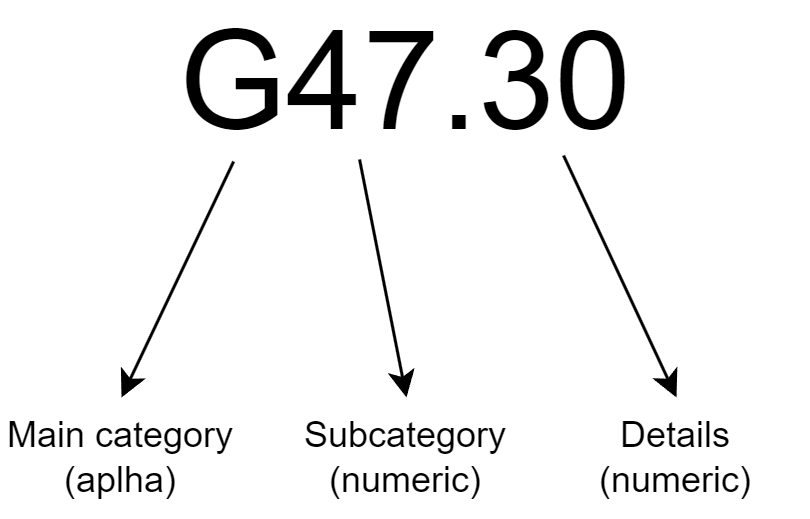
\includegraphics[width=0.8\textwidth]{images/ICD-10-CM.png}
	
	\caption{Structure of MKCH-10 code.}
	\label{fig:icd-10-cm}
\end{figure}

This code consists of three parts, as shown in Fig. \ref{fig:icd-10-cm}. The first part is a letter that encodes the main categories of diseases, also known as chapters. For example, codes starting with G represent diseases of the nervous system. Following this, there are two numeric characters that further specify the subcategory of the disease, such as codes from G40 to G47, which are episodic and paroxysmal disorders, with G47 specifically being sleep disorders. We observe that episodic and paroxysmal disorders only extend up to G47, meaning that theoretically, subgroups G48 and G49 could exist with a 4 in the second position but would not belong to the same G4 subcategory as G40 or G47 \label{mkch_subdiv}. Fortunately, this is not the case; when a higher-level subcategory (like G4) does not have 10 lower-level subcategories (like G47), these subcategories do not exist at all. If there are more than 10 lower-level subcategories, they are assigned multiple consecutive higher-level subcategories, such as disorders of other endocrine glands, which span from E20 to E35. The code then contains a dot, after which there are characters that further describe the details of the disease, such as etiology, anatomic site, and severity. According to the official documentation, ICD-10-CM codes can be up to 7 characters long, meaning that after the first three characters specifying the category, there can be up to 4 additional alphanumeric characters to further specify the disease \cite{icd10expl}. However, the version used in Slovak healthcare database, MKCH-10, contains only up to two numeric characters to specify the disease \cite{mkch10expl}. These details are organized such that the first position conveys higher-level information than the second; for example, G47.3 is sleep apnea, and G47.30 is primary central sleep apnea.
\\

To embed this code, we first split it into its three parts and separately embed each part. We then concatenated the embeddings of each part to obtain the final disease embedding. For the main category, we generated random vectors from a uniform distribution for each letter in the English alphabet (representing all main categories). We chose random vectors to ensure relatively similar distances between any two main categories, as there are no inherent relationships among these categories. We also considered using one-hot encoding, which would make the distance between every pair of categories identical, but opted against it because this approach would constrain the vector length.
\\

In embedding the second part, which is the subcategory, we used a different approach. For each number between 00 and 99 (all possible values of this part), we assigned a linearly spaced number within a chosen interval. This value was then repeated multiple times to create a vector. This repetition was implemented to encode the importance of this part of the code. This approach has both advantages and disadvantages. The advantage is that we can be sure that closely related disease subgroups, like G46 and G47, would receive similar embeddings since their subgroup codes are close on the number line. However, there are also two disadvantages. The first is that G49 and G50 would be similarly close as G46 and G47, but fortunately, in most cases, either the X9 code does not exist at all, creating a gap, or if the X9 code exists it belongs to a category that goes past X as a higher-level subgroup. Another disadvantage is that the distance between two higher-level subgroups can vary quite dramatically, even though in reality there might not be a reason for such a difference. For example, using this approach, the higher-level subgroup G40–G47 is much closer to subgroup G50–G59 than to G80–G83.
\\

Finally, to embed details, we used the same approach as for subgroups, since these codes function similarly. The only difference was that not all codes included second-level details. In such cases, we added "5" as a proxy value to minimize the average distance from all potential codes sharing the same first-level detail code (with second-level information) while maximizing the average distance to codes with different first-level details.
\\

Once all parts were embedded, we created the final embedding by concatenating them. To encode the importance of each part, we assigned different vector lengths. This works because each value in the vector has the same mean and variance. We encoded the importance hierarchically: the main category received the longest embedding, subgroups a medium length, and details the shortest embedding.

\subsection{Drug embedding}
\label{drugEmb}

Similarly to diagnosis, to embed drug information we used the international code associated with each drug. In the case of drugs, this was the Anatomical Therapeutic Chemical (ATC) classification system. Like the MKCH-10 code, the ATC code can be split into multiple parts, with each subsequent part providing more detailed information. The ATC code consists of five parts or levels.
\\

Structure of the ATC code:

\begin{itemize}
	\item First level: A single letter representing one of 14 main anatomical or pharmacological groups (e.g., "C" for cardiovascular system). These groups are shown in Fig. \ref{fig:atc_l1}.
	\item Second level: A two-digit number specifying a pharmacological or therapeutic subgroup (e.g., "C03" for diuretics).
	\item Third and fourth levels: Each uses a single letter to further classify pharmacological, therapeutic, or chemical subgroups (e.g., "C03C" for high-ceiling diuretics and "C03CA" for sulfonamide derivatives).
	\item Fifth level: A two-digit number identifying the specific chemical substance (e.g., "C03CA01" for furosemide).
\end{itemize}

\begin{figure}[!h]
	\centering
	
	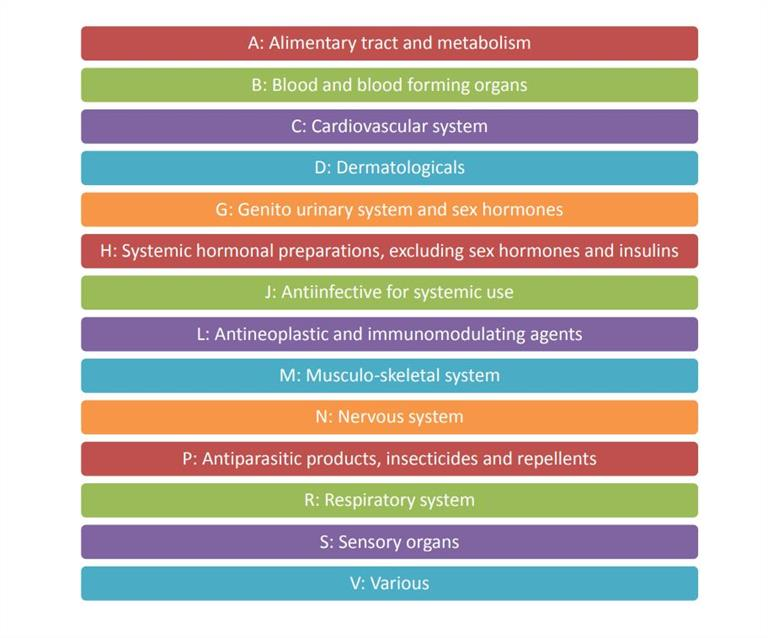
\includegraphics[width=0.8\textwidth]{images/atc_l1_classification_who.jpg}
	
	\caption{Fourteen main anatomical or pharmacological groups and their corresponding first level ATC code \cite{atc_who}.}
	\label{fig:atc_l1}
\end{figure}

Embedding was performed in a manner very similar to the diagnosis embedding: each level was embedded separately, and the final embedding was created by concatenating them. In this case, each level was embedded using a random vector drawn from a uniform distribution. We chose random vectors because none of the ATC levels contain internal subgroupings analogous to the hierarchical subgroups seen in diagnosis codes (see \ref{mkch_subdiv} for subgroup code details). To encode the importance of each level, we again varied the lengths of the random vectors. This approach ensures that the similarity between codes depends more on matches in the lower, more important levels than in the higher ones.
\\

\subsection{Medical procedure embedding}
\label{procedureEmb}

The final component to embed was medical procedures. In this case, no structured code is implemented within the Slovak healthcare system. To address this, we embedded textual descriptions of procedures using two approaches:

\begin{itemize}
	\item Multilingual Large Language Model (LLM): We selected the LaBSE model (section \ref{theoryLaBSE}), trained on multiple languages including Slovak. LaBSE generates similar embeddings for semantically equivalent sentences across languages, which aligns with medical terminology often being international.
	\item Slovak-specific Word2Vec: A Word2Vec model (section \ref{theoryW2v}) trained exclusively on Slovak textual data.
\end{itemize}

For both methods, we reduced the dimensionality of the resulting embeddings using Principal Component Analysis (PCA) to eliminate low-variance dimensions encoding minimal information.
\\

To construct the final record embedding, we concatenated all four components (timestamp, diagnosis, medical procedure, and prescribed drug). Since timestamp and diagnosis are always available, we substituted missing drug or procedure data with zero vectors of matching length. This neutral substitution preserves compatibility between datasets while maintaining centered embeddings.

\section{Prediction of future number of records}

Our task is to get information about how much will cost patient in the future, more specifically, how much it will cost in the next. Since our approach predicts future records, assign to them cost and sum the cost into resulting cost, we need to somehow be able to assess how many records need to be generated in order to simulate approximately next year. For this task we tried two different approaches.
\\

First approach was to predict approximate number of records using linear regression which gets counts of records from previous years and predict next one. Other approach used stopping criterion, which uses timestamp information which is available in each input and generated records, and stop generating once difference between last timestamp from patient data and last generated timestamp surpass one year threshold.
\\

Each of these method have it's own disadvantages. In case of linear regression, number of records per year can vary significantly, so even though we expect increase \cite{num_of_vis} regression might not be able to catch this trend, especially if patient data consist of only few years in the past. Potential issue with second approach is that it's dependent on how well model learned that timestamp should always increase.  

% !TeX spellcheck = en_EN-English

\section{Future record prediction}
\label{record_prediction}

%This task is both the most important and the most challenging to train. Our goal is to develop a model capable of predicting a patient's potential next record based on their previous ones. Generally, this task is nearly impossible with the amount of information available, as numerous factors influence whether, when, and what new disease a patient might contract, how their current state will evolve, and what specific actions a doctor will take.
%\\

This task is both the most important and the most challenging to train. Our goal is to develop a model capable of predicting a patient’s potential next record based on their previous ones. In general, this is nearly impossible given the available information, as many other factors influence if, when, and what new disease a patient might contract, how their condition will evolve, and what actions a doctor will take.
\\

Fortunately, our ultimate goal is not to predict a patient's specific future but to estimate the likely total cost of their future records. We anticipate that even if we cannot predict exact outcomes, we can still estimate the overall cost.
\\

To achieve this prediction, we experimented with multiple models. The first three models we tested were Recurrent Neural Networks (RNNs): multi-layer Elman RNN, multi-layer Gated Recurrent Unit (GRU) RNN, and multi-layer Long Short-Term Memory (LSTM) RNN. The architecture of these models is detailed in Sec. \ref{theoryRNN}. The last model we tried was a Transformer, specifically a Decoder-only Transformer model, explained in Sec. \ref{theoryTrans}.



% !TeX spellcheck = en_EN-English

\section{Record cost prediction}
\label{recCostPred}

The next step in total cost prediction involves estimating the cost of individual records. This is necessary because the future records we predict lack cost information, requiring an additional model to determine it. We adopted this approach to leverage the entire record for prediction, rather than relying solely on a single cost dimension that could have been added. For this task, we selected a standard Multilayer Perceptron (MLP), a multi-layered, fully-connected feed-forward neural network, whose architecture is detailed in Sec. \ref{MLP}.
\\

We also trained a Gradient Boosting model and a Ridge regression model for comparative analysis. These were chosen to represent two distinct model families: decision trees (Gradient Boosting) and linear regression (Ridge). We selected these specific representatives because they employ more sophisticated techniques than base models in their respective groups and have demonstrated performance comparable to, if not better than, artificial neural networks in similar studies, such as the work by Mohammad Amin Morid et al. \cite{morid2018supervised} (discussed in Chap. \ref{simStudy}).
% !TeX spellcheck = en_EN-English

\chapter{Software Design} \label{chap:softwaredesign}

This chapter is dedicated to introducing the software used to create, train, validate, and use the machine learning model described in this thesis. The entire code was written in Python, more specifically in \texttt{Python 3.11.4}. We chose this language for its ease of use and wide selection of libraries for data processing and machine learning. All scripts are available in the GitHub repository at \url{https://github.com/MarianK-py/diploma_thesis_code}.
\\

The code can be divided into three parts:

\begin{enumerate}
	\item Embedding – code to create embedding mapping files
	\item Model training and validation – code to set up, train, validate, and save prediction models, this needs to be run once
	\item Predictor – code to load trained models and predict the future cost of inputted patients
\end{enumerate}

The code for model training and validation, and the code for prediction, use the same technologies, which is why they are described in a single section. Now we will introduce the libraries and pre-trained models used in our code: first those used in general, and then those specific to each part mentioned above.

\section{General}

Some of the libraries were used in all parts of the code to maintain coherence in the technologies used.
\\

In this category belongs the \texttt{Pandas 2.2.1} library, a fast, powerful, flexible, and easy-to-use open-source data analysis and manipulation tool \cite{pandas}, which was used to load, manipulate, and save all datasets. Another is the \texttt{Numpy 1.26.4} library, an open-source project that enables numerical computing with Python \cite{numpy}. We used it for computations such as random number generation, calculation of mean and standard deviation for data normalization, and many other tasks.

% !TeX spellcheck = en_EN-English

\section{Embedding}
\label{embedDesign}

For embedding we used couple additional libraries since we utilized couple of algorithms and pre-trained models. More specifically libraries and specific algorithms and models we used are these: 
\\

\begin{itemize}
	\item \texttt{Scikit-learn 1.2.2} - simple and efficient tools for predictive data analysis \cite{scikitlearn},  we specifically use function to compute PCA in order to decrease dimensionality of medical procedure embedding and function K-means clustering in order to check embedding has desired property
	
	\item \texttt{NTLK}
	
	\item \texttt{Simplemma}
	
	\item \texttt{SentenceTransformer}
	
	\item \texttt{Gensim}
\end{itemize}



Simplemma (lemmatizer)

sentence transformers (LaBSE)

gensim (word2vec)

ntlk (word tokenizer)

% !TeX spellcheck = en_EN-English
\newpage

\section{Model training, validation and prediction}
\label{modelDesign}

For training, validation, and using models for predictions, we primarily used \texttt{PyTorch 2.6.0}, which is an optimized tensor library for deep learning using GPUs and CPUs \cite{pytorch}. This library provided us with all the required components, such as linear, non-linear, and specialized layers, to assemble both simpler neural networks like the MLP (used for prediction of the cost category of a record) and more complex neural networks like LSTM or Transformer (used to predict future records). In addition to the building blocks for the networks themselves, PyTorch also offers other components needed for model training, such as optimizers and loss functions, with the possibility to modify them for our specific requirements, as we did for the loss function used in future record prediction.
\\

Another library used here was \texttt{Scikit-learn 1.2.2}, from which we used the linear regression model. We considered this as one possible way to determine how many future records we should generate for a patient to estimate their expected amount for the next year.
% !TeX spellcheck = en_EN-English

\chapter{Implementation} \label{chap:implementation}


% !TeX spellcheck = en_EN-English

\section{Embedding of Patient}
\label{embeddingImple}

The first sub-task in predicting a patient’s future costs is to embed each patient record into a numerical vector that can be interpreted by a neural network. For each patient record, four types of information are embedded. The first and easiest to implement is the timestamp, which is computed using numerical and date values. The other three, which are more complex, are the diagnosis, medical procedure, and prescribed drug.

\subsection{Timestamp}
\label{timespampImple}

To compute the timestamp, we first gathered all records for a single patient and identified the one with the earliest date. This record served as a pivot for calculating all timestamps for the patient. To compute the timestamp for this initial record, we took the patient's age in years, added half a year, and then multiplied by 365 to obtain an approximate age in days, which served as the timestamp. We added half a year to improve the approximation, as we only have the age in years and do not know whether the patient's birthday occurred one or eleven months ago, however, we assumed it to be on average six months, or half a year. For all subsequent records, we calculated the difference in days between the record date and the date of the first record, and then added this difference to the timestamp from the first record to create the timestamp for each subsequent record.

\subsection{Diagnosis embedding}

As discussed in Sec. \ref{diagEmb}, the embedding of diagnoses is based on the MKCH-10-SK (ICD-10-CM) code of the disease. We split this code into three parts, embed each part independently, and finally concatenate the results.
\\

To embed the main category, we generated a vector containing random numbers using a uniform distribution for each letter of the English alphabet. We chose to sample these random numbers from the interval [-0.5, 0.5]. This interval was chosen mostly arbitrarily, as we planned to pass the resulting embedding into a normalization function once it was complete.
\\

For the subcategory and details, we linearly assigned a value to each possible two-digit code. We chose the interval for these values to be [-0.5, 0.5], meaning subcategory 00 would get -0.5, category 50 would get 0, and category 99 would get 0.5. This interval was chosen so that each dimension of this embedding would have the same mean and standard deviation as each dimension of the main category. As a result, each position in each part of the embedding contributes equally to the total distance, allowing us to use the number of dimensions to weigh each part of the code.
\\

The most important part was to assign lengths to the vector of each part in a way that would encode their importance. The main category, the most important part, got a vector of length 28, the subcategory part got length 7, and finally, the details got length 3.
\\

A showcase of the resulting embedding can be seen in Fig. \ref{fig:diag_emb_show}, where each part is highlighted by a different color and all values are rounded to two decimals.

\begin{figure}[!h]
	\centering
	
	% TODO image needs update after change of lengths of each embeddings
	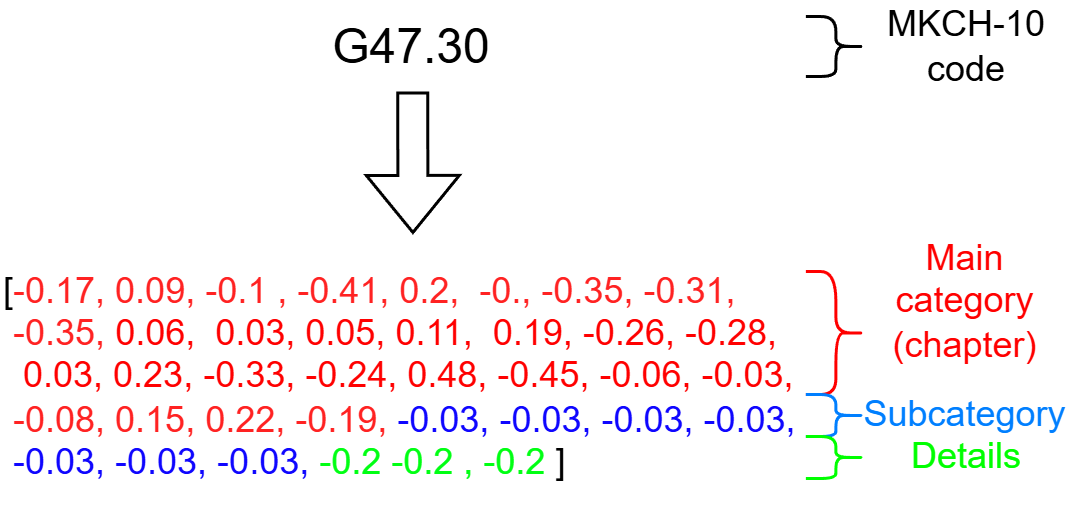
\includegraphics[width=0.8\textwidth]{images/diagnosis_embed_showcase.png} 
	
	\caption{Showcase of resulting embedding of specific diagnosis (rounded to two decimal places).}
	\label{fig:diag_emb_show}
\end{figure} 


\subsection{Drug embedding}

The embedding for drugs was performed similarly to the diagnosis embedding: each level was embedded separately, and the final embedding was created by concatenating them. For drug codes, each level was embedded using a random vector sampled from a uniform distribution over the interval [-0.5, 0.5]. We chose random vectors because none of the ATC levels contain internal subgroupings analogous to the hierarchical subgroups in diagnosis codes (see Sec. \ref{mkch_subdiv}). To encode the importance of each level, we again varied the vector lengths, with higher levels (e.g., anatomical groups) assigned shorter vectors. The specific vector lengths for each level are provided in Tab. \ref{tab:drug_lev_len}, resulting in a total embedding length identical to the diagnosis embedding. If a code is incomplete (i.e., missing higher levels), the missing parts are replaced with zero vectors, which act as neutral elements in the embedding space.
\\

\begin{table}[!h]
	\centering
	\begin{tabular}{|l|l|}
		\hline
		Level  & Length \\ \hline
		1 & 21 \\ \hline
		2 & 9 \\ \hline
		3 & 5 \\ \hline
		4 & 2 \\ \hline
		5 & 1 \\ \hline
	\end{tabular}
	\caption{Lengths of random vectors assigned to each information level of ATC code.}
	\label{tab:drug_lev_len}
\end{table}  

With this embedding, we should obtain codes whose similarity is more dependent on whether the lower, more important levels match than the higher ones.

\subsection{Medical procedure embedding}

Embedding of medical procedures was straightforward since we used an already trained model.
\\

As discussed in Sec. \ref{procedureEmb}, for the LLM we chose the LaBSE model. It is a model developed by Google to encode text into high-dimensional vectors. This model was trained on 109 languages, including Slovak. Using this model was straightforward, as we just had to input the complete description of the procedure to receive a 768-dimensional dense encoding of it. After computing all embeddings, we performed principal component analysis (PCA) to reduce the dimensionality of this embedding while maintaining most of the variance, or in other words, most of the information stored inside it.
\\

We also tried a different approach using a Word2vec model trained specifically for the Slovak language. More specifically, we used the word2vec-sk model made by the company Essential Data \cite{w2v}. This model was trained on a corpus containing around 110 million words. We chose the version of the model trained using the CBOW approach. Since this model is trained to embed words and not text, we first split the description of the procedure into words and lemmatized those words, in other words, changed them into their base form. Then, using the Word2vec model, we embedded each word into a dense 200-dimensional vector separately and finally created the description embedding as an average of the embeddings of all words in it.
\\

We expected that the LaBSE model would produce better results compared to standard text embedding models trained solely on the Slovak language, since the LaBSE model is trained by comparing embeddings not only to similar sentences in Slovak but also to their translations in other languages. This could mitigate the relatively small amount of Slovak language data compared to other, more commonly used languages. Additionally, this model could recognize domain-specific words, in our case medical terms, which are often left in a foreign language and would most likely not be found in a Slovak-only corpus.
\\

As mentioned in Sec. \ref{embedding}, the final embedding was created by concatenating all four parts and filling any missing parts with zeros, which serve as a neutral substitution.

% !TeX spellcheck = en_EN-English

\chapter{Research} \label{chap:research}


% !TeX spellcheck = en_EN-English

\section{Embedding of patient}
\label{embeddingRes}

First of sub-tasks for prediction of patient future costs is to embed each patient record into numerical vector that would be understandable for neural network. For each record of a patient we embed four information. First and easy to implement is a timestamp which is computed using numerical and date values, then there three more tricky information and those are diagnosis, medical procedure and prescribed drug. 


\subsection{Diagnosis embedding}

We need to confirm that closely related diagnosis would get embedding with smaller distance meaning higher similarity compared to less related diagnosis.
In order to confirm that our embedding has desired properties we computed similarity of embedding of multiple codes. As similarity function we choose simple multiplicative inverse of Euclidean distance. In table \ref{tab:diag_emb_show} we can see results. Highest similarity was between codes G47.30 and G40.09 which is expected since they belong to same main category and very close subcategory, second highest was between H40.09 and H18.80 which are only other combination that belong to same main category, this confirms that main category has biggest impact since this similarity is significantly higher than that between G40.09 and H40.09 which differ only main category.

\begin{table}[!h]
	\centering
	\begin{tabular}{|l|l|l|}
		\hline
		Code A & Code B & Similarity \\ \hline
		G47.30 & G40.09 & 2.77       \\ \hline
		G47.30 & H40.09 & 0.53       \\ \hline
		G47.30 & H18.80 & 0.46       \\ \hline
		G40.09 & H40.09 & 0.54       \\ \hline
		G40.09 & H18.80 & 0.45       \\ \hline
		H40.09 & H18.80 & 0.84       \\ \hline
	\end{tabular}
	\caption{Similarities of embedding of multiple chosen MKCH-10 codes}
	\label{tab:diag_emb_show}
\end{table}  

Another confirmation that embeddings works as intended by clustering them. More specifically we would expect that if we group embeddings into as many clusters as are main categories, each cluster should contain mostly if not only diagnosis from one main category. On order to test this we used K-means clustering with 26 clusters which is number of different main categories of diagnosis and got these results:

\begin{table}[!h]
	\begin{tabular}{|p{0.15\textwidth}|p{0.2\textwidth}|p{0.5\textwidth}|}
		\hline
		Cluster ID & Cluster size & Frequency of first level values \\ \hline
		0 & 654 & C: 654, \\ \hline
		1 & 2092 & M: 2092, \\ \hline
		2 & 766 & Y: 766, \\ \hline
		3 & 543 & S: 543, \\ \hline
		4 & 786 & Z: 786, \\ \hline
		5 & 1100 & T: 1100, \\ \hline
		6 & 1067 & X: 1067, \\ \hline
		7 & 620 & H: 496, U: 124, \\ \hline
		8 & 752 & S: 752, \\ \hline
		9 & 1770 & M: 1770, \\ \hline
		10 & 739 & Q: 739, \\ \hline
		11 & 584 & D: 584, \\ \hline
		12 & 507 & F: 507, \\ \hline
		13 & 958 & W: 958, \\ \hline
		14 & 556 & E: 556, \\ \hline
		15 & 491 & A: 491, \\ \hline
		16 & 553 & O: 553, \\ \hline
		17 & 627 & K: 627, \\ \hline
		18 & 872 & V: 872, \\ \hline
		19 & 521 & G: 521, \\ \hline
		20 & 463 & L: 463, \\ \hline
		21 & 420 & R: 420, \\ \hline
		22 & 465 & B: 465, \\ \hline
		23 & 717 & J: 319, P: 398, \\ \hline
		24 & 568 & I: 568, \\ \hline
		25 & 535 & N: 535, \\ \hline
\end{tabular}
\end{table}

In table we can see that almost every cluster consist of diagnosis from with only single main category. Only immediately visible issues are clusters 7 and 23 where two main categories got assigned same cluster which is most likely caused by their small size compared to other and by the fact that largest categories M and S got split into two clusters.

\subsection{Drug embedding}

To confirm this we do similar check as we did with diagnosis code and compute similarity of four chosen ATC codes and see if our theory holds. To compute similarity we again use multiplicative inverse of Euclidean distance. We choose C01EB15, C01CA04, C10AA07 and J01CA04, we would expect first two to be most similar since they match on first levels, than first two compared to third should have slightly lower similarity since they match on only first level and finally we expect that all three would be least similar to fourth one since first level is different, even though that second and forth match on all other levels.  We can see results in table \ref{tab:drug_emb_show}. We can see that results met our expectation with highest similarity between first two and lowest between any of first three and fourth, even in case of second and forth that match on all other levels except first.

\begin{table}[!h]
	\centering
	\begin{tabular}{|l|l|l|}
		\hline
		Code A & Code B & Similarity \\ \hline
		C01EB15 & C01CA04 & 1.24      \\ \hline
		C01EB15 & C10AA07 & 0.54       \\ \hline
		C01EB15 & J01CA04 & 0.45       \\ \hline
		C01CA04 & C10AA07 & 0.64       \\ \hline
		C01CA04 & J01CA04 & 0.48       \\ \hline
		C10AA07 & J01CA04 & 0.38       \\ \hline
	\end{tabular}
	\caption{Similarities of embedding of multiple chosen ATC codes}
	\label{tab:drug_emb_show}
\end{table}  

Also similarly to diagnosis we can test whether our embeddings would cluster mainly first level of code or not. Since there are 14 main anatomical or pharmacological groups \ref{fig:atc_l1} we used K-means algorithm with 14 clusters and got these results:


\begin{table}[!h]
	\begin{tabular}{|p{0.15\textwidth}|p{0.2\textwidth}|p{0.5\textwidth}|}
		\hline
		Cluster ID & Cluster size & Frequency of first level values \\ \hline
		0 & 8645 & C: 8645, \\ \hline
		1 & 19132 & N: 19132, \\ \hline
		2 & 9322 & L: 8657, S: 665, \\ \hline
		3 & 11734 & A: 11734, \\ \hline
		4 & 7159 & B: 7159, \\ \hline
		5 & 9526 & V: 9526, \\ \hline
		6 & 4681 & R: 4681, \\ \hline
		7 & 14732 & C: 14732, \\ \hline
		8 & 7237 & V: 7237, \\ \hline
		9 & 4031 & M: 3987, P: 44, \\ \hline
		10 & 3599 & G: 3599, \\ \hline
		11 & 2367 & N: 2367, \\ \hline
		12 & 9032 & D: 1266, G: 897, H: 1136, J: 5733, \\ \hline
		13 & 6093 & N: 6075, P: 18, \\ \hline
\end{tabular}
\end{table}

We can see that clusters mostly consist of embeddings with same first level values. There are some exceptions which are most likely caused by uneven number of drug in each category. Because of this categories with smallest number of drug like P, S, D, H or G got assigned to cluster along with bigger category and categories with biggest number of drugs like N, C or V got split into multiple categories.  

\subsection{Medical procedure embedding}




% !TeX spellcheck = en_EN-English

\chapter{Results} \label{chap:results}

In this chapter, we will report and discuss the training and testing of the models we identified as the best performing on the training subset of data in Sec. \ref{costPredRes} and Sec. \ref{recordPredRes}, now trained on the complete training dataset.
\\

\section{Training of final models}
\label{modelTrain}

Both MLP and Decoder-only Transformer models were trained on a dataset consisting of 156 020 patients (approximately 90\% of all patients in our complete dataset). Each model was trained for 10 epochs.
\\

For the MLP model, we settled on a batch size of 512 and an initial learning rate of 0.0004. After the final epoch, the model achieved a training loss of 0.0303 and a training accuracy of 80.2\%, indicating a slight improvement over the model trained on the subset of data. However, the improvement is so minor that it suggests either reaching the upper limit of extractable information from the data or an unidentified flaw in our approach.
\\

For the Decoder-only Transformer model, we used a lookback value of 20, meaning the model always processed the last 20 patient records to predict the 21st record. Due to the increased input size, we used a significantly smaller batch size of 64 compared to the MLP model. The initial learning rate was set to 0.0025. Training with these parameters resulted in a final training loss of 0.4005, which is significantly lower than the 0.5200 training loss of the model trained on the subset.

\section{Validation of trained models}
\label{modelValid}

Validation of the models was performed using a dataset containing records of 16 335 patients, accounting for over 9\% of our total patient population.
\\

In the case of the MLP model for cost prediction, we obtained a validation loss of 0.0305 and an accuracy of 80.1\%. Both loss and accuracy improved compared to the model trained on a subset of the data, which had a loss of 0.0349 and an accuracy of 78\%. However, these differences are relatively small. Additionally, the validation loss and accuracy are on par with the training metrics, indicating that the model does not suffer from overfitting.
\\

In our application, we ultimately won't use the cost categories of predicted records as they are but will aggregate them into a single category per patient. If the model occasionally predicts a category that is off by one in either direction, the final results will be affected only slightly, as there is a high likelihood that these errors might offset each other. Therefore, if we consider the percentage of cases where the model predicted either the precise category or one off, we achieve an adjusted accuracy of 96.8\% (and 99.2\% if we allow the model to be off by two categories). 
\\

Another interesting statistic to examine is the model's accuracy in each cost category to ensure it can predict correctly across all categories, not just those with the majority of the data. Here, accuracy is defined as the ratio of records successfully assigned to a category relative to all records that should belong to that category.  The results of this check can be seen in Tab. \ref{tab:cat_acc}, where we observe that accuracy declines with the frequency of categories in the dataset. However, despite the low frequency of categories 5 to 7, the model still achieves over 50\% accuracy, and only two categories (8 and 9) have accuracy below 50\%, which together form a very small part of the dataset (less than 0.4\%).
\\

\begin{table}[!h]
	\centering
	\begin{tabular}{|l|l|l|}
		\hline
		Category & Dataset frequency & Validation accuracy \\ \hline
		1        & 34.7\%           & 87.5\%              \\ \hline
		2        & 37.6\%           & 84.4\%              \\ \hline
		3        & 15.0\%           & 62.5\%              \\ \hline
		4        & 7.0\%            & 54.8\%              \\ \hline
		5        & 3.3\%            & 53.7\%              \\ \hline
		6        & 1.1\%            & 50.8\%              \\ \hline
		7        & 0.9\%            & 58.1\%              \\ \hline
		8        & 0.2\%            & 35.3\%              \\ \hline
		9        & 0.2\%            & 38.2\%              \\ \hline
	\end{tabular}
	\caption{Accuracies of record cost prediction model in each possible prediction category.}
	\label{tab:cat_acc}
\end{table}
 
For the Decoder-only Transformer model trained to predict future records, the final validation loss was 0.4740. This is significantly better than the validation loss of 0.6212 for the same model trained on the subset of data and matches or exceeds the training errors of all other model configurations tested during hyperparameter tuning.
\newpage

\section{Testing of patient future cost prediction}
\label{pat_fut_res}

The last 1,000 patients, who were not used in either training or validation, were employed to test whether the combination of trained models could succeed in our primary task: predicting the cost of a patient for the next year.
\\

Since the cost for an entire year can be significantly larger than the cost for a single record, we decided to adjust the intervals for categories accordingly. The intervals for patient costs can be seen in Tab. \ref{tab:patCost}, where we adopted an approach in which the threshold for the next category is approximately double that of the previous one.
\\

\begin{table}[!h]
	\centering
	\begin{tabular}{|l|l|}
		\hline
		Category  & Interval \\ \hline
		1 & $\interval[{0,100})$ \\ \hline
		2 & $\interval[{100,200})$ \\ \hline
		3 & $\interval[{200,500})$ \\ \hline
		4 & $\interval[{500,1000})$ \\ \hline
		5 & $\interval[{1000,2000})$ \\ \hline
		6 & $\interval[{2000,5000})$ \\ \hline
		7 & $\interval[{5000,10000})$ \\ \hline
		8 & $\interval[{10000,20000})$ \\ \hline
		9 & $\interval[{20000,\infty})$ \\ \hline
	\end{tabular}
	\caption{Intervals of patient cost for each category.}
	\label{tab:patCost}
\end{table}  

Under normal circumstances, the workflow for computing a patient’s future cost would look like this:

\begin{enumerate}
	\item Load patient data.
	\item Embed patient records.
	\item Compute the number of future records.
	\item Predict the given number of future records.
	\item Predict the cost of future records.
	\item Transform the sum of future record costs into the patient’s future cost category.
\end{enumerate}

However, since we aim to test our model, we modify this workflow slightly. After loading patient data, records from the last year are separated from the rest and are not seen by the model. Using the remaining records, the model predicts costs based on the predefined workflow. Afterwards, the cost is extracted from the separated records, and the real cost category of the patient for that year is compared to the model’s predictions to assess accuracy or proximity.
% !TeX spellcheck = en_EN-English

\chapter*{Conclusion}

This thesis set out to address the challenge of predicting the future costs for patients within the Slovak healthcare system, using underutilized medical data available. The primary objective was to develop a machine learning framework capable of forecasting patient expenses for the following year, using historical records of medical procedures and drug prescriptions.
\\

To achieve this, the work was divided into several key tasks: embedding patient records into meaningful numerical vectors, predicting future medical events, estimating the costs of these events, and aggregating these predictions to forecast annual patient expenses. A variety of models were explored, including multilayer perceptrons (MLP), recurrent neural networks (RNNs) such as LSTM, and decoder-only Transformer architectures. Special attention was devoted to the design of embeddings for diagnoses, drugs, and procedures, ensuring that similar medical events would have similar representations, thereby improving the models’ predictive capabilities.
\\

In the embedding tasks, the desired results were achieved, especially for medical procedures. Based on our evaluations, the resulting embeddings can be used for clustering procedures into groups, a capability for which no practical solution currently exists. While the approach did not yield perfect results, we believe that with further refinement, it could become suitable for production use.
\\

The results for predicting patient future cost categories showed that the approach works reasonably well. The model managed to get the exact cost category right in 39.9\% of cases, and was within one category in 84.4\% of cases.
\\

However, the analysis also revealed limitations. The model tended to underestimate costs, particularly for patients with records in higher-cost categories. This is likely due to class imbalance and the inherent difficulty of predicting rare, high-expense events.
\\

Despite these challenges, the thesis demonstrates that it is possible to use routinely collected healthcare data to forecast future patient costs with decent precision. The framework developed here could help healthcare providers and policymakers with planning resources, identifying high-risk patients earlier, and managing care more efficiently.
\\

In summary, this thesis demonstrates that advanced machine learning methods can improve predictive analytics in healthcare. There’s definitely room for improvement, especially as more and better data becomes available, but we believe this work is a step towards more personalized and data-driven healthcare in Slovakia and possibly elsewhere.





%main content 


% -------------------
% --- Bibliografia
% -------------------

\backmatter

\nocite{*}
\bibliographystyle{plain}
\bibliography{references}

%---koniec bibliografie

\end{document}